%%% LaTeX Template: Two column article
%%%
%%% Source: http://www.howtotex.com/
%%% Feel free to distribute this template, but please keep to referal to http://www.howtotex.com/ here.
%%% Date: February 2011

%%% Preamble
\documentclass[	DIV=calc,%
							paper=a4,%
							fontsize=12pt,%
							onecolumn]{scrartcl}	 					% KOMA-article class

\usepackage{lipsum}													% Package to create dummy text
\usepackage[english]{babel}										% English language/hyphenation
\usepackage[protrusion=true,expansion=true]{microtype}				% Better typography
\usepackage{amsmath,amsfonts,amsthm}					% Math packages
\usepackage[pdftex]{graphicx}									% Enable pdflatex
\usepackage[svgnames]{xcolor}									% Enabling colors by their 'svgnames'
\usepackage[hang, small,labelfont=bf,up,textfont=it,up]{caption}	% Custom captions under/above floats
\usepackage{epstopdf}												% Converts .eps to .pdf
\usepackage{subfig}													% Subfigures
\usepackage{booktabs}												% Nicer tables
\usepackage{fix-cm}													% Custom fontsizes
\usepackage[utf8]{inputenc}
\usepackage[top=2.5cm, bottom=2.5cm, left=2.5cm, right=2.5cm]{geometry}
\usepackage[ddmmyyyy]{datetime}
\usepackage{verbatim}
\addto\captionsenglish{%
	\renewcommand\tablename{Tabela}
	\renewcommand\figurename{Figura}
} 
 

 
%%% Custom sectioning (sectsty package)
\usepackage{sectsty}													% Custom sectioning (see below)
\allsectionsfont{%															% Change font of al section commands
	\usefont{OT1}{phv}{b}{n}%										% bch-b-n: CharterBT-Bold font
	}

\sectionfont{%																% Change font of \section command
	\usefont{OT1}{phv}{b}{n}%										% bch-b-n: CharterBT-Bold font
	}



%%% Headers and footers
\usepackage{fancyhdr}												% Needed to define custom headers/footers
	\pagestyle{fancy}														% Enabling the custom headers/footers
\usepackage{lastpage}	

% Header (empty)
\lhead{}
\chead{}
\rhead{}
% Footer (you may change this to your own needs)

%% ====================================
%% ====================================
%% mude o rodape  do projeto
%% ====================================
%% ====================================

\lfoot{\footnotesize \texttt{Cabeamento Estruturado - Redes VI} \textbullet ~Certificação}


\cfoot{}
\rfoot{\footnotesize página \thepage\ de \pageref{LastPage}}	% "Page 1 of 2"
\renewcommand{\headrulewidth}{0.0pt}
\renewcommand{\footrulewidth}{0.4pt}



%%% Creating an initial of the very first character of the content
\usepackage{lettrine}
\newcommand{\initial}[1]{%
     \lettrine[lines=3,lhang=0.3,nindent=0em]{
     				\color{DarkGoldenrod}
     				{\textsf{#1}}}{}}



%%% Title, author and date metadata
\usepackage{titling}															% For custom titles

\newcommand{\HorRule}{\color{DarkGoldenrod}%			% Creating a horizontal rule
									  	\rule{\linewidth}{1pt}%
										}

\pretitle{\vspace{-25pt} \begin{flushleft} \HorRule 
				\fontsize{50}{50} \usefont{OT1}{phv}{b}{n} \color{DarkRed} \selectfont 
				}

%% ====================================
%% ====================================
%% mude o titulo  do projeto
%% ====================================
%% ====================================

\title{Projeto de Cabeamento Estruturado para Edifício de dois Andares}					% Title of your article goes here

%% ====================================



\posttitle{\par\end{flushleft}\vskip 0.5em}

\preauthor{\begin{flushleft}
					\large \lineskip 0.5em \usefont{OT1}{phv}{b}{sl} \color{DarkRed}}
\author{Augusto Fernando Ruis, Clayton Camargo Oliveira, Leonardo Jambersi, João Emiliano dos Santos, Renan Ribeiro Sakomoto Zuculin e Rodrigo Dall' Agnol}  	% Author name goes here


\postauthor{\footnotesize \usefont{OT1}{phv}{m}{sl} \color{Black} 
					\\Universidade Tecnológica Federal do Paraná - Câmpus Cornélio Procópio 								% Institution of author
					\par\end{flushleft}\HorRule}

\date{}																				% No date




%%% Begin document
\begin{document}
\maketitle
\thispagestyle{fancy} 	
\thispagestyle{empty}		% Enabling the custom headers/footers for the first page 
% The first character should be within \initial{}




%% ====================================
%% ====================================
%% mude o resumo  do projeto
%% ====================================
%% ====================================
\initial\textbf{Esta documentação tem como objetivo demonstrar na prática a elaboração de um projeto de cabeamento estruturado, embasando-se em normas nacionais e internacionais como, por exemplo, NBR-14565-2007 e TIA/EIA-568-B. A implantação do presente projeto será realizado de forma fictícia em um edifício comercial de dois andares, onde o piso 1 possui 6 salas e o piso 2 possui 10 salas com tomadas de telecomunicações.
A rede de cabeamento estruturado será criada do zero com o intuito de administrar de uma forma precisa e eficaz os recursos de dados e voz, atendendo as necessidades momentâneas e futuras de uma organização.
Os elementos de rede presente nos pisos serão devidamente identificados utilizando-se de padrões, o layout se dá por meio de um cabeamento horizontal que interliga cada área de trabalho aos armários de telecomunicações presentes nos dois pisos e esses por sua vez são interligados por um backbone.}

%% ====================================
%%\begin{figure}
%%	\centering
%%	\includegraphics{utfpr}
%%\end{figure}

\vspace{2cm}
\centerline{\textit{\textbf{\today}}}

\clearpage
    \renewcommand*\listfigurename{Lista de figuras}
\listoffigures

\renewcommand*\listtablename{Lista de tabelas}
\listoftables




\clearpage
\renewcommand{\contentsname}{Sumário}
\tableofcontents
\clearpage

%% ====================================
%% ====================================
%% Inicio do texto
%% ====================================
%% ====================================
\section{Introdução}
O projeto tem a finalidade de atender a necessidade de interligação de dois andares, sendo o piso 1 com 6 salas e o piso 2 com 10 salas, levando pontos de redes com acesso a dados e voz, por meio de cabeamento horizontal para cada área de trabalho do edifício. 
Atualmente o prédio não conta com nenhum equipamento de TI facilitando a implantação do projeto em questão.
Basicamente o projeto utilizará um armário de telecomunicação em cada piso interligados por um backbone e em cada armário de telecomunicação teremos um path panel e switch para dados e um path panel e switch para voz.


\subsection{Benefícios}
Com a implantação de um projeto de cabeamento estruturado seguindo normas como NBR-14565-2007 e TIA/EIA-568-B os principais benefícios são:
\begin{itemize}
\item Probabilidade de ocorrer erros na camada física é menor por conta dos equipamentos e testes realizados no processo;
\item A identificação de problemas posteriores na camada física podem ser localizados de forma mais fácil por conta da identificação dos pontos de redes;
\item Uma rede estruturada esta preparada para um processo de ampliação. 
\end{itemize}

\section{Usuários}
A estrutura contará inicialmente com 16 tomadas de telecomunicação distribuídas nas salas do piso 1, onde as salas 1 e 4 terão 4 tomadas cada uma e as demais salas terão 2 tomadas cada.
O piso 2 contará com 23 tomadas de telecomunicação sendo que a sala 2 possuirá 3 tomadas e a sala 3 possuirá 4 tomadas, as demais sala do piso terão duas tomadas de telecomunicação cada uma.
A maioria das salas possuem 2 tomadas pois para o processo de certificação essa é a quantidade mínima de pontos para cada área de trabalho, porém a estrutura final contará com a possibilidade de ampliação da rede como um todo, visto que a empresa possui metas de crescimento e o projeto de cabeamento estruturado visa atender essa expansão.


\section{Estrutura predial existente}
A estrutura a ser atendida com o projeto de cabeamento estruturado é composta por 2 pisos. O piso 1 possui área de 278,00 metros, dividido em 6 salas e o piso 2 possui área de 278,00 metros, dividido em 10 salas, sendo que ambos possuem estrutura para passagem do cabeamento, como eletrocalhas, canaletas, dutos e caixas de passagem. As figuras 1 e 2 ilustram a planta do piso 1 e 2 respectivamente    

%% Figura 1 piso 1
\begin{figure}
	\centering
	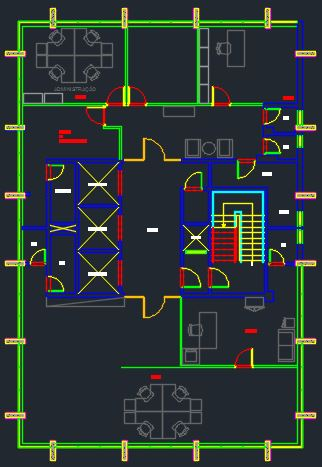
\includegraphics[]{piso1}
	\caption{Planta Piso 1}
	\label{fig1}
\end{figure}

%% Figura 2 piso 2
\begin{figure}
	\centering
	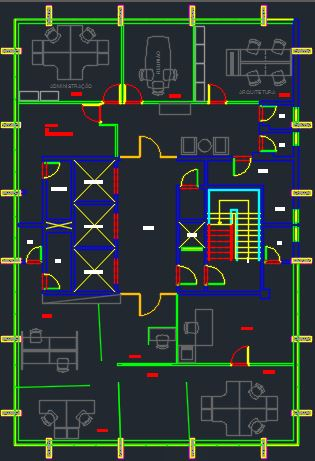
\includegraphics[]{piso2}
	\caption{Planta Piso 2}
	\label{fig2}
\end{figure}


\section{Planta Lógica - Elementos estruturados}

\subsection{Topologia}
No piso 1 foi inserido um armário de telecomunicações, que contém dois Path Panels de 24 portas, e esses estão diretamente conectados a dois Switches de 24 portas. Esses equipamentos estão divididos da seguinte maneira um Switch e um Path Panel disponível para dados e um Switch e um Path Panel disponível para voz e uma régua de energia, todos esses equipamentos estão localizados em um rack de 24U 670mm, disponibilizando um total de 32 pontos de comunicação, dividindo-se em dezesseis para dados e dezesseis para voz, interconectando as seis salas presentes nesse piso.
No piso 2 foi inserido um armário de telecomunicações, que contém dois Path Panels de 48 portas, e esses estão diretamente conectados a dois Switches de 48 portas. Esses equipamentos estão divididos da seguinte maneira um Switch e um Path Panel disponível para dados e um Switch e um Path Panel disponível para voz e uma régua de energia, todos esses equipamentos estão localizados em um rack de 24U 670mm, disponibilizando um total de 46 pontos de comunicação, dividindo-se em vinte e três para dados e vinte e três para voz, interconectando as dez salas presentes nesse piso. A interligação dos pavimentos utiliza-se de um backbone composto de fibra óptica 2 pares.
A tabela 1 ilustra o layout dessa topologia acima descrita e a tabela 2 é a legenda dos equipamentos apresentados na tabela 1.

\begin{table}[h!]
\centering
\caption{Diagrama Lógico de rede}
\label{tab1}
\begin{tabular}{|l|l|l|}
\hline
\multicolumn{1}{|l|}{Armários de Telecomunicação} \\ \hline
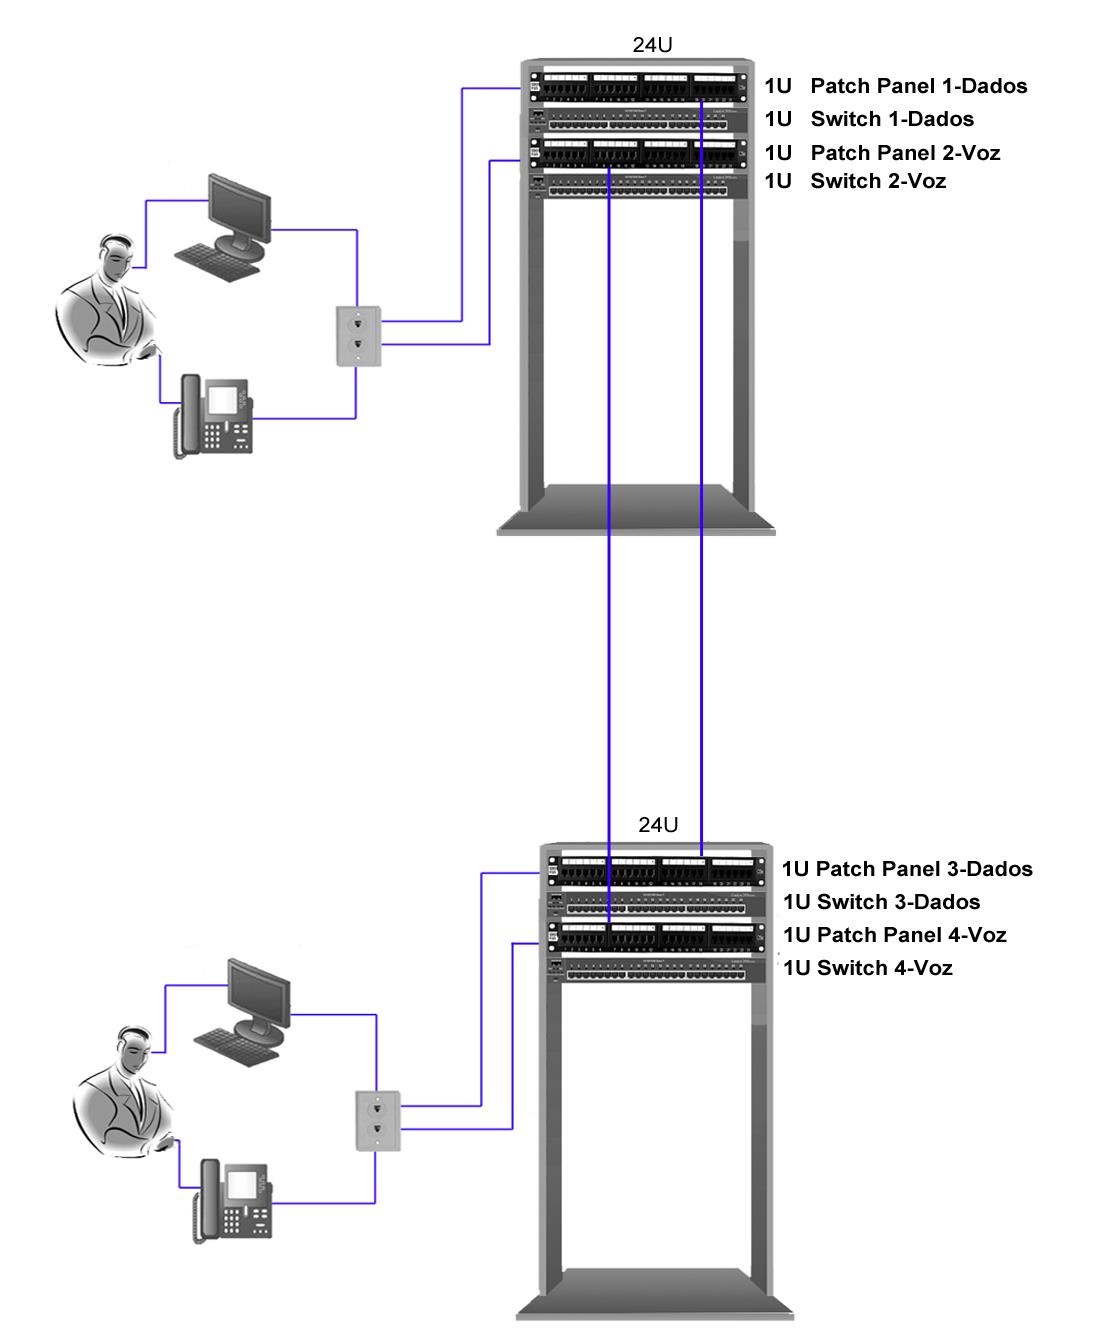
\includegraphics[scale=0.2]{fig1}        \\ \hline

\end{tabular}
\end{table}
\begin{table}[h!]
\centering
\caption{Legenda dos Equipamentos}
\label{tab2}
\begin{tabular}{|l|l|l|}
\hline
\multicolumn{1}{|l|}{Descrição dos Materiais} \\ \hline
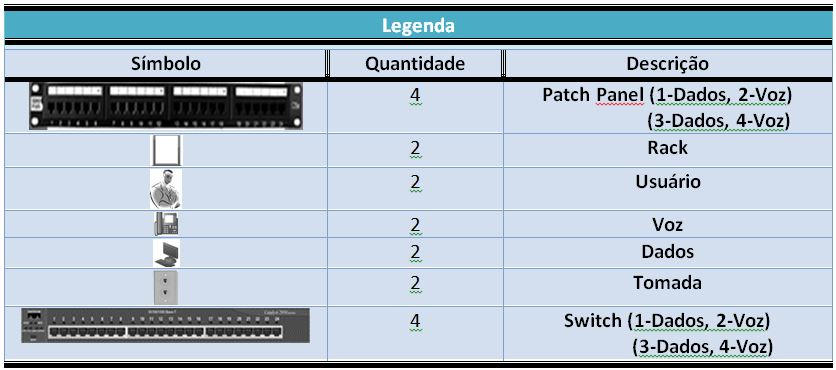
\includegraphics[scale=0.5]{fig2}        \\ \hline

\end{tabular}
\end{table}

\subsection{Encaminhamento}
O cabeamento foi realizado em dois pisos de um edifício comercial, utilizando-se de eletrocalhas embutidas na parede, as tomadas de telecomunicações que disponibilizam dados e voz estão a 45 cm do chão conforme as normas de cabeamento estruturado.

\subsection{Memorial descritivo}
Na tabela 3 temos os principais equipamentos que serão utilizados para a elaboração do projeto com a estimativa de quantidade, abaixo da tabela segue as especificações dos equipamentos de maior relevância.
\begin{table}[h!]
\centering
\caption{Quantidade dos Equipamentos}
\label{tab3}
\begin{tabular}{|l|l|l|}
\hline
\multicolumn{1}{|l|}{Principais Equipamentos} \\ \hline
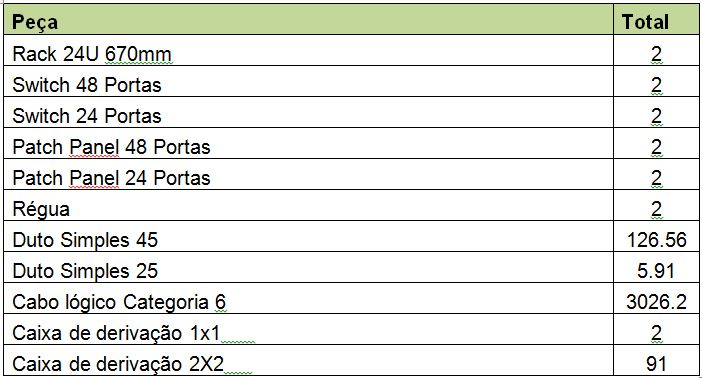
\includegraphics[scale=0.5]{fig3}        \\ \hline

\end{tabular}
\end{table}

A figura 3 apresenta o Armário de telecomunicação utilizado no piso 1 e 2, com as seguintes especificações: 
\begin{itemize}
\item Material: Aço
\item Espessura: 2,00 mm
\item Espessura Portas e Laterais: 1,20 mm
\item Altura: 2100 mm
\item Largura: 600 mm
\item Profundidade: 800mm
\item Peso: 112Kg
\end{itemize}

%% Figura 3 rack
\begin{figure}
\centering
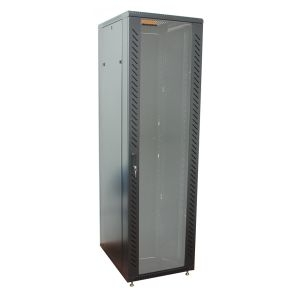
\includegraphics[]{rack}
\caption{Rack Fechado 19 44U x 600 x 800 mm para Piso Preto Nazda }
\label{fig3}
\end{figure}


Figura 4 apresenta Switch de 48 portas utilizado no piso 2 para atender as 10 salas presentes no andar.
O Cisco Catalyst 3550 12G é um membro da série Catalyst 3550G Switches Ethernet Inteligentes, uma linha de classe empresarial, empilhável, multilayer switches que fornecem alta disponibilidade, segurança e qualidade de serviço (QoS) para melhorar o funcionamento da rede. Com uma gama de configurações Fast Ethernet e Gigabit Ethernet, a série Catalyst 3550G pode servir tanto como switch de camada de um poderoso acesso para armários de ligações médias empresas e como um switch de backbone para redes de médio porte.

%% Figura 4 switch 48 portas
\begin{figure}
	\centering
	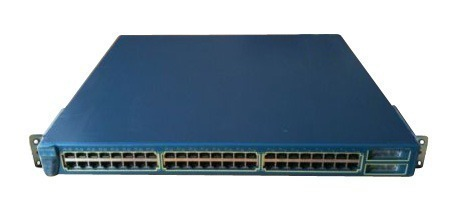
\includegraphics[]{sw48}
	\caption{Switch Cisco 48 Portas Catalyst Ws-c3550}
	\label{fig4}
\end{figure}


Figura 5 apresenta Switch de 24 portas utilizado no piso 1 para atender as 6 salas presentes no andar.
Switch Baseline com Configuração fixa - 24 portas Gigabit 10/100/1000 que suportam conexões de alto desempenho.
Priorização IEEE 802.1p que oferece compatibilidade com as redes que suportam aplicações de tempo real.
Pode ser montado em racks ou empilhado para otimizar o espaço, sua altura de 1U padrão simplifica o planejamento do espaço.

%% Figura 5 switch 24 portas
\begin{figure}
	\centering
	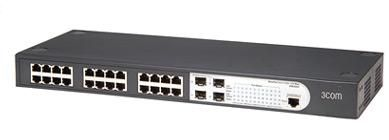
\includegraphics[]{sw24}
	\caption{Switch Gigabit 3com 24 Portas 10/100/1000 }
	\label{fig5}
\end{figure}


Figura 6 apresenta Path Panel de 24 e 48 portas utilizados nos armários de telecomunicação que interliga o cabeamento horizontal aos Switches.
\begin{itemize}
\item Excede os requisitos estabelecidos nas normas para CAT.6 / Classe E
\item Performance garantida para até 6 conexões em canais de até 100 metros
\item 24 ou 48 posições RJ-45
\item Painel frontal em plástico com porta etiquetas para identificação
\item Possui borda de reforço para evitar empenamento 
\item Fornecido com parafusos e arruelas para fixação
\item Fornecido com ícones de identificação e velcros para organização
\item Fornecido com guia traseiro para melhor organização dos cabos
\end{itemize}

%% Figura 6 path panel 24/48 portas
\begin{figure}
	\centering
	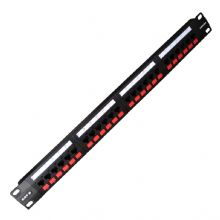
\includegraphics[]{pp2448}
	\caption{Patch Panel 24 e 48 portas}
	\label{fig6}
\end{figure}


Figura 7 apresenta a régua utilizado nos armários de telecomunicação com a seguinte característica: 
\begin{itemize}
\item Régua sem disjuntor com 8 tomadas para rack e cabo com 1,5 mts
\end{itemize}

%% Figura 7 regua
\begin{figure}
	\centering
	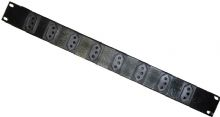
\includegraphics[]{regua}
	\caption{Régua com 8 tomadas}
	\label{fig7}
\end{figure}


\subsection{Identificação dos cabos}
A tabela 4 representa a identificação dos pontos das 6 salas presentes no piso 1.
A tabela 5 representa a identificação dos pontos das 10 salas presentes no piso 2, com a seguinte legenda:
\begin{itemize}
\item TO - Número da tomada de telecomunicação
\item A  - Dados 
\item B  - Voz	
\item SL - Sala 
\item P  - Piso
\end{itemize}

%% Tabelas com identificação dos Pontos
\begin{table}[]
\centering
\caption{Identificação dos pontos Piso 1}
\label{my-label}
\begin{tabular}{|l|l|l|l|l|}
\hline
\textbf{USUÁRIO} & \textbf{LOCAL} & \textbf{TIPO DE SERVIÇO} & \textbf{IP} & \textbf{PORTA PONTO} \\ \hline
Sala1 & Sala Administração & Ponto de Dados & 172.16.0.2 & TO1ASL1P1 \\ \hline
Sala1 & Sala Administração & Ponto de Voz & 10.0.0.2 & TO1BSL1P1 \\ \hline
Sala1 & Sala Administração & Ponto de Dados & 172.16.0.3 & TO2ASL1P1 \\ \hline
Sala1 & Sala Administração & Ponto de Voz & 10.0.0.3 & TO2BSL1P1 \\ \hline
Sala1 & Sala Administração & Ponto de Dados & 172.16.0.4 & TO3ASL1P1 \\ \hline
Sala1 & Sala Administração & Ponto de Voz & 10.0.0.4 & TO3BSL1P1 \\ \hline
Sala1 & Sala Administração & Ponto de Dados & 172.16.0.5 & TO4ASL1P1 \\ \hline
Sala1 & Sala Administração & Ponto de Voz & 10.0.0.5 & TO4BSL1P1 \\ \hline
Sala2 & Sala2 & Ponto de Dados & 172.16.0.6 & TO5ASL2P1 \\ \hline
Sala2 & Sala2 & Ponto de Voz & 10.0.0.6 & TO5BSL2P1 \\ \hline
Sala2 & Sala2 & Ponto de Dados & 172.16.0.7 & TO6ASL2P1 \\ \hline
Sala2 & Sala2 & Ponto de Voz & 10.0.0.7 & TO6BSL2P1 \\ \hline
Sala3 & Sala3 & Ponto de Dados & 172.16.0.8 & TO7ASL3P1 \\ \hline
Sala3 & Sala3 & Ponto de Voz & 10.0.0.8 & TO7BSL3P1 \\ \hline
Sala3 & Sala3 & Ponto de Dados & 172.16.0.9 & TO8ASL3P1 \\ \hline
Sala3 & Sala3 & Ponto de Voz & 10.0.0.9 & TO8BSL3P1 \\ \hline
Sala4 & Sala4 & Disponível – Dados & 172.16.0.10 & TO9ASL4P1 \\ \hline
Sala4 & Sala4 & Ponto de Voz & 10.0.0.10 & TO9BSL4P1 \\ \hline
Sala4 & Sala4 & Disponível – Dados & 172.16.0.11 & TO10ASL4P1 \\ \hline
Sala4 & Sala4 & Ponto de Voz & 10.0.0.11 & TO10BSL4P1 \\ \hline
Sala4 & Sala4 & Disponível – Dados & 172.16.0.12 & TO11ASL4P1 \\ \hline
Sala4 & Sala4 & Ponto de Voz & 10.0.0.12 & TO11BSL4P1 \\ \hline
Sala4 & Sala4 & Disponível – Dados & 172.16.0.13 & TO12ASL4P1 \\ \hline
Sala4 & Sala4 & Ponto de Voz & 10.0.0.13 & TO12BSL4P1 \\ \hline
Sala5 & copa & Disponível –Dados & 172.16.0.14 & TO13ASL5P1 \\ \hline
Sala5 & copa & Ponto de Voz & 10.0.0.14 & TO13BSL5P1 \\ \hline
Sala5 & copa & Disponível –Dados & 172.16.0.15 & TO14ASL5P1 \\ \hline
Sala5 & copa & Ponto de Voz & 10.0.0.15 & TO14BSL5P1 \\ \hline
Sala6 & Ponto Extra & Disponível -Dados & 172.16.0.16 & TO15ASL6P1 \\ \hline
Sala6 & Ponto Extra & Ponto de Voz & 10.0.0.16 & TO15BSL6P1 \\ \hline
Sala6 & Ponto Extra & Disponível -Dados & 172.16.0.17 & TO16ASL6P1 \\ \hline
Sala6 & Ponto Extra & Ponto de Voz & 10.0.0.17 & TO16BSL6P1 \\ \hline
\end{tabular}
\end{table}
\begin{table}[]
\centering
\caption{Identificação dos pontos Piso 2}
\label{my-label}
\begin{tabular}{|l|l|l|l|l|}
\hline
\textbf{USUÁRIO} & \textbf{LOCAL} & \textbf{TIPO DE SERVIÇO} & \textbf{IP} & \textbf{PORTA PONTO} \\ \hline
Sala1 & Sala Administração & Ponto de Dados & 172.16.0.18 & TO1ASL1P2 \\ \hline
Sala1 & Sala Administração & Ponto de Voz & 10.0.0.18 & TO1BSL1P2 \\ \hline
Sala1 & Sala Administração & Ponto de Dados & 172.16.0.19 & TO2ASL1P2 \\ \hline
Sala1 & Sala Administração & Ponto de Voz & 10.0.0.19 & TO2BSL1P2 \\ \hline
Sala2 & Sala de Reunião & Ponto de Dados & 172.16.0.20 & TO3ASL2P2 \\ \hline
Sala2 & Sala de Reunião & Ponto de Voz & 10.0.0.20 & TO3BSL2P2 \\ \hline
Sala2 & Sala de Reunião & Ponto de Dados & 172.16.0.21 & TO4ASL2P2 \\ \hline
Sala2 & Sala de Reunião & Ponto de Voz & 10.0.0.21 & TO4BSL2P2 \\ \hline
Sala2 & Sala de Reunião & Ponto de Dados & 172.16.0.22 & TO5ASL2P2 \\ \hline
Sala2 & Sala de Reunião & Ponto de Voz & 10.0.0.22 & TO5BSL2P2 \\ \hline
Sala3 & Sala Arquitetura & Ponto de Dados & 172.16.0.23 & TO6ASL3P2 \\ \hline
Sala3 & Sala Arquitetura & Ponto de Voz & 10.0.0.23 & TO6BSL3P2 \\ \hline
Sala3 & Sala Arquitetura & Ponto de Dados & 172.16.0.24 & TO7ASL3P2 \\ \hline
Sala3 & Sala Arquitetura & Ponto de Voz & 10.0.0.24 & TO7BSL3P2 \\ \hline
Sala3 & Sala Arquitetura & Ponto de Dados & 172.16.0.25 & TO8ASL3P2 \\ \hline
Sala3 & Sala Arquitetura & Ponto de Voz & 10.0.0.25 & TO8BSL3P2 \\ \hline
Sala3 & Sala Arquitetura & Ponto de Dados & 172.16.0.26 & TO9ASL3P2 \\ \hline
Sala3 & Sala Arquitetura & Ponto de Voz & 10.0.0.26 & TO9BSL3P2 \\ \hline
Sala4 & Sala4 & Disponível - Dados & 172.16.0.27 & TO10ASL4P2 \\ \hline
Sala4 & Sala4 & Ponto de Voz & 10.0.0.27 & TO10BSL4P2 \\ \hline
Sala4 & Sala4 & Disponível - Dados & 172.16.0.28 & TO11ASL4P2 \\ \hline
Sala4 & Sala4 & Ponto de Voz & 10.0.0.28 & TO11BSL4P2 \\ \hline
Sala5 & Sala5 & Disponível -Dados & 172.16.0.29 & TO12ASL5P2 \\ \hline
Sala5 & Sala5 & Ponto de Voz & 10.0.0.29 & TO12BSL5P2 \\ \hline
Sala5 & Sala5 & Disponível -Dados & 172.16.0.30 & TO13ASL5P2 \\ \hline
Sala5 & Sala5 & Ponto de Voz & 10.0.0.30 & TO13BSL5P2 \\ \hline
Sala6 & Sala6 & Disponível -Dados & 172.16.0.31 & TO14ASL6P2 \\ \hline
Sala6 & Sala6 & Ponto de Voz & 10.0.0.31 & TO14BSL6P2 \\ \hline
Sala6 & Sala6 & Disponível -Dados & 172.16.0.32 & TO15ASL6P2 \\ \hline
Sala6 & Sala6 & Ponto de Voz & 10.0.0.32 & TO15BSL6P2 \\ \hline
Sala7 & Sala7 & Disponível -Dados & 172.16.0.33 & TO16ASL7P2 \\ \hline
Sala7 & Sala7 & Ponto de Voz & 10.0.0.33 & TO16BSL7P2 \\ \hline
Sala7 & Sala7 & Disponível -Dados & 172.16.0.34 & TO17ASL7P2 \\ \hline
Sala7 & Sala7 & Ponto de Voz & 10.0.0.34 & TO17BSL7P2 \\ \hline
Sala8 & Sala8 & Disponível -Dados & 172.16.0.35 & TO18ASL8P2 \\ \hline
Sala8 & Sala8 & Ponto de Voz & 10.0.0.35 & TO18BSL8P2 \\ \hline
Sala8 & Sala8 & Disponível -Dados & 172.16.0.36 & TO19ASL8P2 \\ \hline
Sala8 & Sala8 & Ponto de Voz & 10.0.0.36 & TO19BSL8P2 \\ \hline
Sala9 & Sala9 & Disponível -Dados & 172.16.0.37 & TO20ASL9P2 \\ \hline
Sala9 & Sala9 & Ponto de Voz & 10.0.0.37 & TO20BSL9P2 \\ \hline
Sala9 & Sala9 & Disponível -Dados & 172.16.0.38 & TO21ASL9P2 \\ \hline
Sala9 & Sala9 & Ponto de Voz & 10.0.0.38 & TO21BSL9P2 \\ \hline
Sala10 & Copa & Disponível -Dados & 172.16.0.39 & TO22ASL10P2 \\ \hline
Sala10 & Copa & Ponto de Voz & 10.0.0.39 & TO22BSL10P2 \\ \hline
Sala10 & Copa & Disponível -Dados & 172.16.0.40 & TO23ASL10P2 \\ \hline
Sala10 & Copa & Ponto de Voz & 10.0.0.40 & TO23BSL10P2 \\ \hline
\end{tabular}
\end{table}


\section{Implantação}
A tabela 6 indica o cronograma para execução das etapas do projeto de cabeamento estruturado, desde a demarcação dos pontos até a finalização do projeto.

\begin{table}[h!]
\centering
\caption{Cronograma de implantação}
\label{tab6}
\begin{tabular}{|l|l|l|}
\hline
\multicolumn{1}{|l|}{} \\ \hline
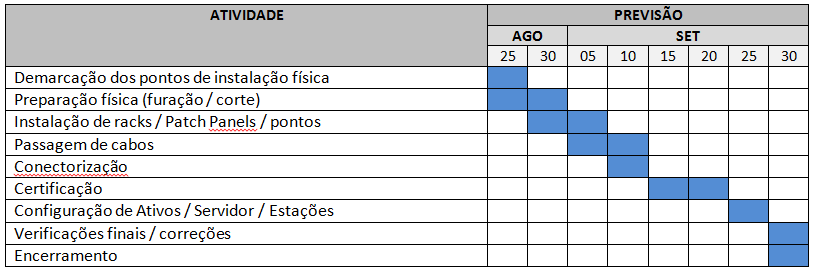
\includegraphics[scale=0.8]{cronograma}        \\ \hline

\end{tabular}
\end{table}

\section{Plano de certificação}
Tão importante quanto à instalação é a certificação de uma rede, que da a garantia que a rede esta disponível para uso. Todos os teste devem ser realizados por profissionais qualificados e equipamentos especiais e devidamente calibrados que seguem uma serie de parâmetros determinados pelas normas.

\begin{itemize}
\item Configuração de Terminação (Wire Map)
\item Comprimento do Cabo
\item Perda de Inserção (Atenuação)
\item Perda de Retorno (Impedância)
\item Paradiafonia NEXT, PS-NEXT, ELNEXT e PS-ELNEXT
\item Relação Atenuação/Paradiafonia (ACR)
\item Atraso de Propagação (Delay)
\item Desvio no Atraso de Propagação (Delay Skew)	
\end{itemize}

A certificação será iniciada após as instalações dos componentes e será realizada em horário comercial. Será realizada a Certificação de toda rede relacionada nesse projeto. 


\section{Plano de manutenção}
Todo material utilizado no cabeamento estruturado devera ser de um único fabricante ou de fabricantes que juntos atendem todas as necessidade e garantias do projeto.  
Deve ser realizada revisão a cada 3 messes no primeiro ano e após primeiro ano a cada 6 messes. 
Dentro de 5 anos serão feitas visitas para revisão da rede e cobrindo garantia e substituição de componentes defeituosos decorrente de causas naturais ou de uso. Visitas extras serão realizadas até 5 dias úteis após solicitação do contratante.  Será realizado certificações a cada 10 novos pontos implantados. 


\section{Referências bibliográficas}
\begin{itemize}
\item ASSOCIAÇÃO BRASILEIRA DE NORMAS TÉCNICAS. NBR 14565: Procedimento básico para elaboração de projetos de cabeamento de telecomunicações para rede interna estruturada. Rio de Janeiro: Abnt – Associação Brasileira de Normas Técnicas, 2000. 48 p.

\item MARIN, Paulo Sérgio. Cabeamento Estruturado: Desenvolvendo cada passo: do projeto à instalação. 3. ed. São Paulo: Érica Ltda., 2010. 336 p.

\item TELECOMMUNICATIONS INDUSTRY ASSOCIATION / ELECTRONIC INDUSTRIES ALLIANCE. 568-B.1-2001: Commercial Building Telecommunications Cabling Standard. Arlington, Va, Estados Unidos: Telecommunications Industry Association 2001, 2001. 79 p.

\end{itemize}


\end{document}